\section{Model Reference Adaptive Control}
\label{c:background} Consider the following nonlinear system in first
order form
\begin{equation}
\label{e:simple:fxu}
\begin{split}
\dot{x}_i &= x_{i+1} \qquad i = 1,2,\cdots,n-1 \\
\dot{x}_n &= f(x,\delta)\\
\delta &= g(x,\deldes),
\end{split}
\end{equation}
where $x \in \dom{x} \subset \real{n}$, is the state of the system,
$\delta \in \real{}$ is the control. The function $f$ represents the
plant dynamics and $g$ represents a state-dependent actuation
nonlinearity. Here, $\deldes \in \real{}$ is the desired actuator
(control) deflection while $\delta$ is the actual deflection.
Typically, $g$ represents actuator magnitude saturation.

The control objective is to synthesize a control law to track a
bounded external command $x_c \in \real{n}$ when $f, g$ are only
approximately known. It is assumed that the full state vector $x$ is
available for feedback. First, the conventional model reference
adaptive control framework is presented for a single input nonlinear
system. The pseudocontrol hedging method is described and used to
protect the adaptive element from incorrect adaptation to input
nonlinearities.

\subsection{Control Design}
Taking the approach of model reference adaptive control
\cite{calise:jgcd:2000}, an approximate model for the plant
dynamics $f(x,\delta)$ may be introduced as
\begin{equation}
\label{e:simple:approx} \nu = \fhat(x,\deldes),
\end{equation}
where $\nu$ is the desired pseudocontrol. For example, in the case
of second order position control of mechanical systems, $\nu$
represents desired acceleration. The function $\fhat(x,\deldes)$ can
be any available approximation of $f(x,\delta)$ with the restriction
that it should invertible with respect to $\deldes$, allowing one to
formulate the dynamic inverse as
\begin{equation}\label{e:simple:inverse}
\deldes = \inv{\fhat}(x,\nu).
\end{equation}
The actuator deflection $\deldes$ is what is expected will achieve
the desired pseudocontrol $\nu$. In introducing these approximate
models and formulation of the controller, it is assumed that the
full state, $x$, is available for feedback. Output feedback
formulations of this architecture are also available
\cite{calise:automatica:2001}. A sufficient condition for
\eq{e:simple:approx} to be invertible is that
$\partial\fhat(x,\delta)/\partial\delta$ is continuous and non-zero
for $(x,\delta) \in \dom{x}\times\real{}$. It is this requirement
that precludes including input saturation nonlinearities as a part
of the inverse.

Substituting the inverse dynamics \eq{e:simple:inverse} into
\eq{e:simple:fxu} results in the following approximately linearized
$n$-integrator system %%
\begin{equation}\label{e:simple:xdot}
\begin{split}
\dot{x}_{i} &= x_{i+1}\qquad i = 1,2,\cdots,n-1\\
 \dot{x}_n &= \nu + \Delbar(x,\delta,\delh) - \nuh,
\end{split}
\end{equation}
where $\delh$ is the an estimate of the actuator position. An
estimate needs to be used when actuator position is not readily
available. If actuator position is measurable then $\delh = \delta$.
The model error is a static nonlinear function and is given by
\[
\Delbar(x,\delta,\delh) = f(x,\delta) - \fhat(x,\delh).
\]
The signal $\nuh$ represents the pseudocontrol that cannot be
achieved due to actuator input characteristics such as saturation and
is given by
\[
\begin{split}
\nuh &= \fhat(x,\deldes) - \fhat(x,\delh) \\
&= \nu - \fhat(x,\delh).
\end{split}
\]
$\nuh$ is also called the pseudocontrol-hedging signal or PCH
signal. This leaves $\nu$, the desired pseudocontrol that may now be
designed to stabilize the linearized system and deal with canceling
the model error $\Delbar$.  The PCH signal, $\nuh$, is a disturbance
and will be dealt with subsequently. Design, $\nu$ to be of the form
\begin{equation}\label{e:simple:nu}
\nu = \nucr + \nulc - \nuhad,
\end{equation}
where $\nucr$ is the output of a reference model, $\nulc$ is the
output of a compensator that stabilizes the linearized dynamics and
$\nuhad$, the output of an adaptive element such as a neural network
that is designed to cancel the effects of model error $\Delbar$.
This architecture is illustrated in \fig{f:mracWithPCH}.
\begin{figure}
  \centering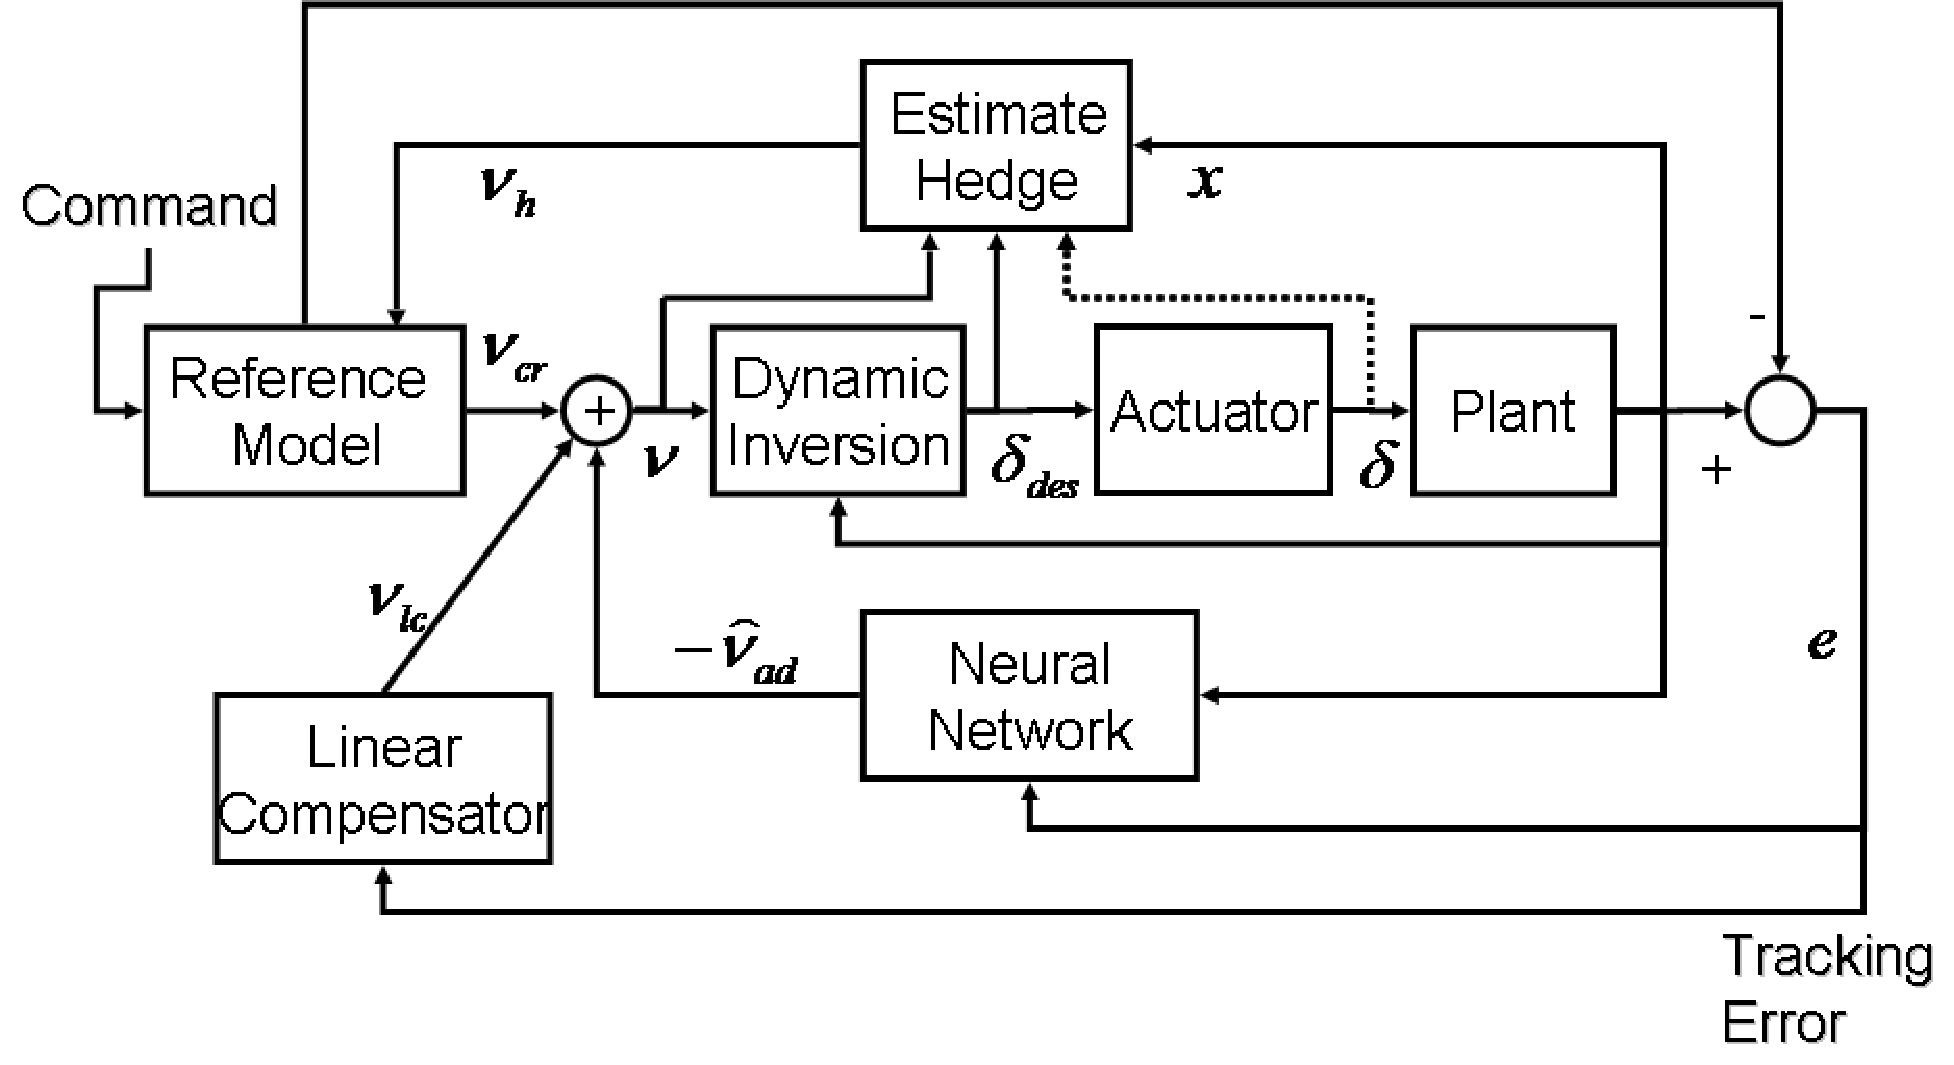
\includegraphics[width=1.0\columnwidth]{arch}
  \caption{Model Reference Adaptive Control Architecture with PCH}
  \label{f:mracWithPCH}
\end{figure}
%
\subsection{Reference Model and Tracking Error} For a system in first order form, the
reference model dynamics may be designed as
\begin{equation}
\begin{split}\label{e:simple:oldrm}
\dot{x}_{r_i} &= x_{r_{i+1}} \qquad i = 1,2,\cdots,n-1\\
\dot{x}_{r_n} &= \nucr(\xr, \xc),
\end{split}
\end{equation}
where $\xr \in \real{n}$ are the states of the reference model and
$\xc \in \real{n}$ is a bounded external command signal. The
reference model tracking error may be defined as
\begin{equation} \label{e:simple:e}
e \triangleq \xr - x.
\end{equation}
When the tracking error dynamics are developed, the form of
\eq{e:simple:oldrm} will result in the $\nuh$ signal appearing as a
part of the error dynamics. Various methods such as anti-windup
synthesis \cite{zaccarian:auto:02} and robustifying terms
\cite{khalil92} may be used to deal with the potentially unbounded
disturbance signal $\nuh$. However, a more critical problem is that
any adaptive element (including a simple integrator) introduced to
cancel the uncertainty $\Delta(\cdot)$ will be trained using the
tracking error signal $e$, and  will attempt to adapt to actuator
nonlinearities due to the presence of $\nuh$ in the tracking error
dynamics. Methods such as anti-windup synthesis and robustifying
terms will leave some element of the input nonlinearity in the
dynamics, thus leading to some amount of incorrect adaptation.

Ultimately, the tracking error dynamics should contain no element of
the saturation nonlinearity, i.e., the signal $\nuh$ must be
completely removed from $\dot{e}$. The PCH method
\cite{ejohnson:phd} is used to protect the adaptive element
from such input characteristics. This may be achieved by augmenting
\eq{e:simple:oldrm} with the hedging signal resulting in the removal
of the actuator characteristic from the tracking error dynamics. The
reference model dynamics are now given by
\begin{equation}
\label{e:simple:rm}
\begin{split}
\dot{x}_{r_i} &= x_{r_{i+1}} \qquad i = 1,2,\cdots,n-1\\
\dot{x}_{r_n} &= \nucr(\xr, \xc) - \nuh.
\end{split}
\end{equation}
If the actuators are saturated then the reference model will
continue to demand tracking as though full authority were still
available resulting in incorrect adaptation. However, the reference
reference model is now "moved" in the opposite direction (hedge) by
an estimate of the amount the plant did not move due to system
characteristics the control designer does not want the adaptive
element to see \cite{ejohnson:phd}.

Note that the PCH signal affects the reference model output, $\nucr$,
only through changes in reference model dynamics and that the
instantaneous pseudocontrol output of the reference model in not
changed. The tracking error dynamics may be found by directly
differentiating \eq{e:simple:e}
\begin{equation*}
\dot{e} =
\begin{bmatrix}
x_{r_2} - x_2 \\
\vdots \\
\dot{x}_{r_n} - \dot{x}_{n}
\end{bmatrix}.
\end{equation*}
%
Considering $\dot{e}_n$,
\begin{equation*}
\begin{split}
\dot{e}_n &= \dot{x}_{r_n} - \dot{x}_{n}\\
          &= \nucr - \nuh - f(x,\delta) \\
          &= \nucr - \nu + \fhat(x,\delh) - f(x,\delta) \\
          &= -\nulc + \nuhad + \fhat(x,\delh) - f(x,\delta)\\
          &= -\nulc - (\Delbar(x,\delta,\delh) - \nuhad).
\end{split}
\end{equation*}
Note that the PCH term, $\nuh$, in \eq{e:simple:rm} cancels the PCH
term in \eq{e:simple:xdot} thus removing it from the tracking error
dynamics. If $\nulc$ is chosen to be a linear compensator of the form
\begin{equation*}
\nulc = \begin{bmatrix}K_1 & K_2 & \cdots & K_n\end{bmatrix}e,
\end{equation*}
%
the overall tracking error dynamics may now be expressed as
\begin{equation}
\label{e:simple:edot} \dot{e} = Ae + B\left[ \nuhad -
\Delbar(x,\delta,\delh)\right],
\end{equation}
where,
\begin{equation*}
A =
\begin{bmatrix}
0      &    1     &    0    &   \cdots    &   0 \\
0      &    0     &    1    &             &   0 \\
\vdots &  \vdots  &         &      \ddots &     \\
0      &    0     &         &             &   1 \\
-K_1   & -K_2     &  -K_3   &     \cdots  &   -K_n
\end{bmatrix},
B =
\begin{bmatrix}
0\\
0\\
\vdots\\
0\\
1
\end{bmatrix},
\end{equation*}
where the compensator gains $K_i$, $i=1,\cdots,n$ are chosen such
that $A$ is Hurwitz. It now remains for $\nuhad$ to be designed to
cancel the model error $\Delbar(x,\delta,\delh)$ and minimize the
forcing term in \eq{e:simple:edot}. Hence the functional form $\nuhad
= \nuhad(x,\delta,\delh)$ is necessary to effectively cancel
$\Delbar$. However $\delta$, the actuator position may not be
measurable leading to the following assumption
\begin{assumption}
\label{ass:simple:ImplicitActuator} The actual actuator position can
be expressed as
\[
\delta = \delta(x,\delh).
\]
For weaker assumptions with regard to the form of the actuator
dynamics see \cite{kannan:phd}.
\end{assumption}
The tracking error dynamics may be represented as
\begin{equation}
\label{e:simple:Trackedot} \dot{e} = Ae + B\left[ \nuhad(x,\delh) -
\Delbar(x,\delh)\right],
\end{equation}
where $\nuhad$ is now only required to be dependent on available
information.

%\section{Adaptive Element}
\label{s:network}
Single hidden layer (SHL) perceptron NNs are
universal approximators\cite{hornik_89,spooner,lewis:ajc:99}. Hence,
given a sufficient number of hidden layer neurons and appropriate
inputs, it is possible to train the network online to cancel model
error.
%
\begin{figure}[h]
  \centering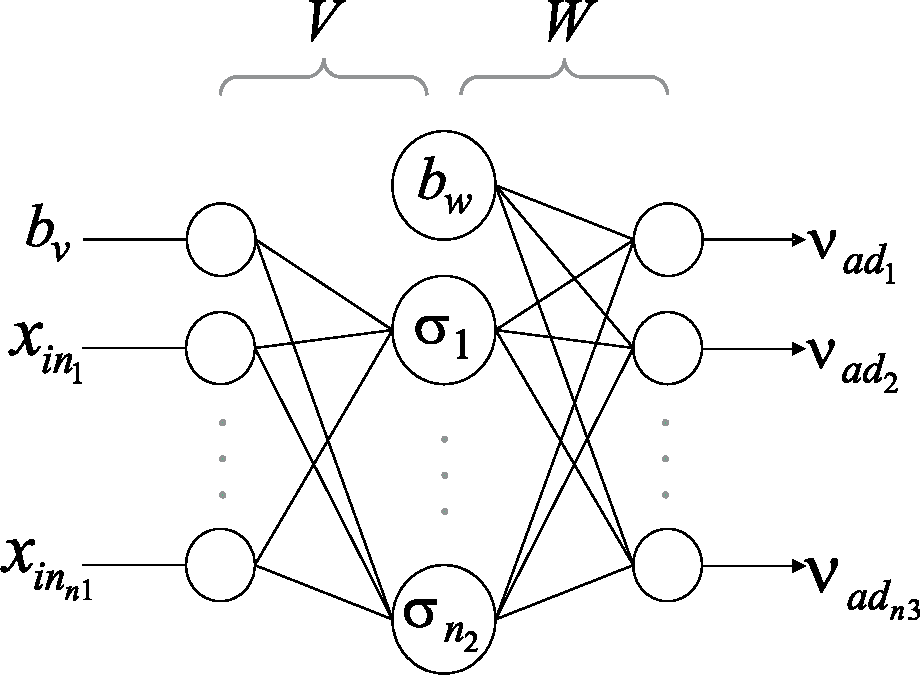
\includegraphics[width=.7\columnwidth]{nn}
%  \centering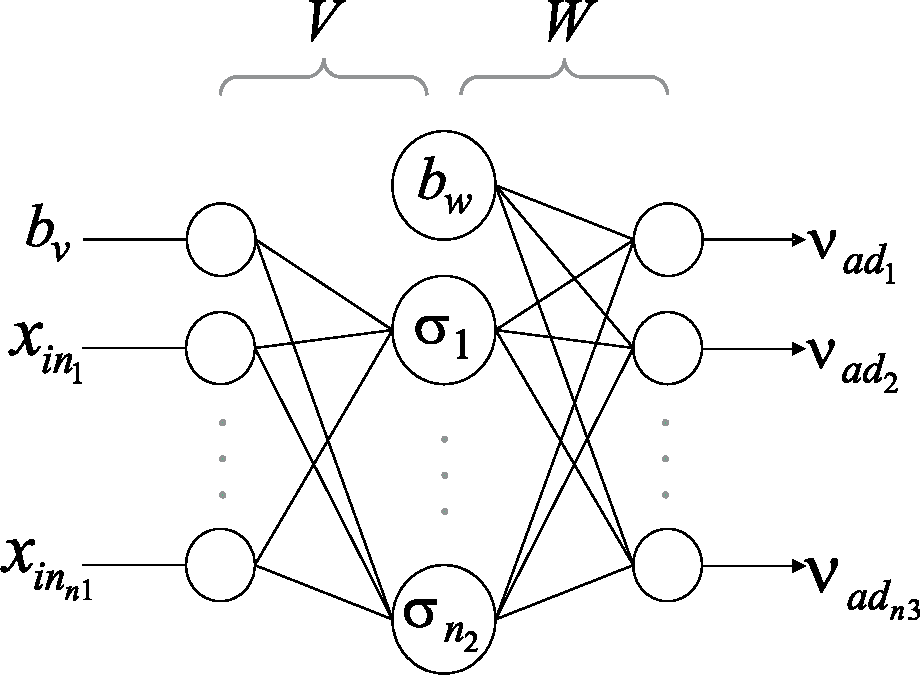
\includegraphics{nn}
  \caption{Neural Network with one hidden layer.}
  \label{f:nn}
\end{figure}
%
\fig{f:nn} shows the structure of a generic single hidden layer
network whose input-output map may be expressed as
\begin{equation}
\nu_{ad_k} = b_w\theta_{w_k} + \sum_{j=1}^{n_2}w_{jk}\sigma_j(z_j),
\end{equation}
where, $k=1,...,n_3$, $b_w$ is the outer layer bias,
$\theta_{w_k}$ is the $k^{th}$ threshold. $w_{jk}$ represents the
outer layer weights, $z_j$ is the input to the neurons, and the scalar $\sigma_j$ is a sigmoidal
activation function
\begin{equation}
\label{e:activation} \sigma_j(z_j) = \frac{1}{1 + e^{-az_j}},
\end{equation}
where, $a$ is the so called \emph{activation potential} and may
have a distinct value for each neuron. $z_j$ is the input to the
$j^{th}$ hidden layer neuron, and is given by
\begin{equation}
z_j = b_v\theta_{v_j} + \sum_{i=1}^{n_1}v_{ij}x_{in_i},
\end{equation}
where, $b_v$ is the inner layer bias and $\theta_{v_j}$ is the
$j^{th}$ threshold. Here, $n_1,n_2$ and $n_3$ are the number of
inputs, hidden layer neurons and outputs respectively. $x_{in_i},
i=1,...,n_1$, denotes the inputs to the NN. For convenience, define
the following weight matrices:
\begin{align}
V &\triangleq
\begin{bmatrix}
\theta_{v,1}    &     \cdots   & \theta_{v,n_2} \\
v_{1,1}         &     \cdots   & v_{1,n_2} \\
\vdots          &     \ddots   & \vdots \\
v_{n_1,1}       &     \cdots   & v_{n_1,n_2}
\end{bmatrix},  \\
W &\triangleq
\begin{bmatrix}
\theta_{w,1}    &     \cdots   & \theta_{w,n_3} \\
w_{1,1}         &     \cdots   & w_{1,n_3} \\
\vdots          &     \ddots   & \vdots \\
w_{n_2,1}       &     \cdots   & w_{n_2,n_3}
\end{bmatrix},  \\
\label{e:Z} Z &\triangleq
\begin{bmatrix}
V   &   0  \\
0   &   W
\end{bmatrix}.
\end{align}
%
Additionally, define the $\bfsigma(\bfz)$ vector as
\begin{equation}
\bfsigma^T(\bfz) \triangleq
\begin{bmatrix}
b_w    &    \sigma(z_1)  &  \cdots &  \sigma(z_{n_2}),
\end{bmatrix}
\end{equation}
where $b_w > 0$ allows for the thresholds, $\bftheta_w$, to be
included in the weight matrix $W$. Also, $\bfz = V^T\bar{\bfx}$,
where,
\begin{equation}
\bar{\bfx}^T =
\begin{bmatrix} b_v   & \bfx_{in}^T
\end{bmatrix},
\end{equation}
where, $b_v > 0$, is an input bias that allows for thresholds
$\bftheta_v$ to be included in the weight matrix $V$.
%
The input-output map of the SHL network may now be written in
concise form as
\begin{equation}
\label{e:nuad} \nuad = W^T\bfsigma(V^T\xbar).
\end{equation}
%
The NN may be used to approximate a nonlinear function, such as
$\Del(.)$. The universal approximation property\cite{hornik_89} of
NN's ensures that given an $\bar{\epsilon} > 0$, then $\forall$
$\xbar \in \domd$, where $\domd$ is a compact set, $\exists$ an
$\bar{n}_2$ and an ideal set of weights $(V^*,W^*)$, that brings the
output of the NN to within an $\epsilon$-neighborhood of the
function approximation error. This $\epsilon$ is bounded by
$\bar{\epsilon}$ which is defined by
\begin{equation}
\bar{\epsilon} = \sup_{\xbar \in \domd} \left\|
W^T\bfsigma(V^T\xbar) - \Del(\xbar) \right\|.
\end{equation}
The weights, $(V^*,W^*)$ may be viewed as optimal values of $(V,W)$
in the sense that they minimize $\bar{\epsilon}$ on $\domd$. These
values are not necessarily unique. The universal approximation
property thus implies that if the NN inputs $\bfx_{in}$ are chosen
to reflect the functional dependency of $\Del(\cdot)$, then
$\bar{\epsilon}$ may be made arbitrarily small given a sufficient
number of hidden layer neurons, $n_2$.

\begin{comment}
\subsubsection{Instantaneous update laws}
 Define $r=e^TPB$, where $P$ is the positive definite solution to the Lyapunov equation as defined in \ref{eq:Lyap}
    \begin{eqnarray}
    \label{eq:backprop_shl}
    \dot{W}=-(\sigma(\bar x)-\sigma'(V^T\bar{x})V^T\bar{x}) r^T \Gamma_W,\\
    \label{eq:backprop_shl_V}
    \dot{V} =  - \Gamma _V \bar xr^TW^T \sigma'(V^T\bar{x}),
    \end{eqnarray}
    where $\Gamma_W,\Gamma_V$ are positive definite matrices that define the learning rate of the NN. This update law closely resembles the backpropagation method of tuning NN weights \cite{Rumelhart:86Nature,Suykens:96bk,Haykin:98bk,Kim:98bk}. However, it is important to note that the training signal $r$ is different from that of the backpropagation based learning laws \cite{Kim:98bk}.
    \end{comment}


The adaptive signal $\nuhad$ actually contains two terms
\begin{equation*}
\nuhad = \nuad + \nur
\end{equation*}
where $\nuad$ is the output of the SHL NN and $\nur$ is a
robustifying signal that arises in the proof of boundedness. The NN
weight matrices may be grouped as
\begin{equation*}
Z \defined \begin{bmatrix}V & 0 \\ 0 & W\end{bmatrix},
\end{equation*} and the weight error is defined as
\begin{equation*}
\tilde{W}\defined W^*-W,\qquad \tilde{V}\defined V^*-V,
\end{equation*}
and correspondingly
\begin{equation*}
\tilde{Z}\defined Z^*-Z.
\end{equation*}
%
%\begin{comment}%
\begin{theorem}[\cite{johnson:phdthesis}]
\label{thm:simple:ebounded} Consider the system given by
\sys{e:simple:fxu} together with the inverse law
\sys{e:simple:inverse} and the following assumptions

\begin{itemize}
\item external command $x_c$ is bounded.
\end{itemize} (
\ref{ass:kcascade:CommandBounded},
\ref{ass:kcascade:NetworkApproxHolds},
\ref{ass:kcascade:IdealWeightsBounded},
\ref{ass:kcascade:FixedPoint}, \ref{ass:kcascade:RefModelBounded}),
with $\bfr, \nuhad, \nuad, \nur$ given by equations
\ref{e:kcascade:r}, \ref{e:kcascade:nuhad},
 \ref{e:kcascade:nuad}, \ref{e:kcascade:nur} respectively. If
$K_r > 0 \in \real{}$ with lower-limit state in the proof, and where
the adaptive laws $\dot{W},\dot{V}$, satisfy
\ref{e:kcascade:Wupdate}, \ref{e:kcascade:Vupdate} with
$\Gamma_W,\Gamma_V > 0$ and scalar $\kappa > 0$ with lower-limit
state in the proof, then, the reference model tracking error,
$\bfe$, and NN weights ($\Wt,\Vt$) are uniformly ultimately bounded.
Further, the plant states, $x$, are uniformly bounded.
\begin{proof}
This theorem is a special case of
\thm{thm:kcascade:simpleBoundedness} with one subsystem. Hence, the
proof given in \secti{s:mainproof} applies and shows boundedness of
$e,\Wt,\Vt$. The external command and command tracking error $e_r$
are bounded by assumption; this implies that all other states are
uniformly bounded. Additionally, see \cite{johnson:phdthesis}.
\end{proof}
\end{theorem}
%\end{comment} 